%%%%%%%%%%%%%%%%%%%%%%%%%%%%%%%%%%%%%%%%%
% University/School Laboratory Report
% LaTeX Template
% Version 3.1 (25/3/14)
%
% This template has been downloaded from:
% http://www.LaTeXTemplates.com
%
% Original author:
% Linux and Unix Users Group at Virginia Tech Wiki 
% (https://vtluug.org/wiki/Example_LaTeX_chem_lab_report)
%
% License:
% CC BY-NC-SA 3.0 (http://creativecommons.org/licenses/by-nc-sa/3.0/)
%
%%%%%%%%%%%%%%%%%%%%%%%%%%%%%%%%%%%%%%%%%

%----------------------------------------------------------------------------------------
%	PACKAGES AND DOCUMENT CONFIGURATIONS
%----------------------------------------------------------------------------------------

\documentclass{article}

\usepackage{graphicx} % Required for the inclusion of images
\usepackage{amsmath} % Required for some math elements
\usepackage{enumitem}
\usepackage{subcaption}
\usepackage{pdfpages}
\usepackage[section]{placeins}

\setlength\parindent{0pt} % Removes all indentation from paragraphs

\renewcommand{\labelenumi}{\alph{enumi}.} % Make numbering in the enumerate environment by letter rather than number (e.g. section 6)

\newlist{inlinelist}{enumerate*}{1}
\setlist*[inlinelist,1]{%
  label=(\arabic*),
}

%----------------------------------------------------------------------------------------
%	DOCUMENT INFORMATION
%----------------------------------------------------------------------------------------

\title{\begin{LARGE}
	\textbf{EE 445L - Lab 6: Introduction to PCB Design}
\end{LARGE}} % Title

\author{Joshua Bryant \\ jmb6357 \and James Morris \\ jsm3288} % Author name

\date{\today} % Date for the report

\begin{document}

\maketitle % Insert the title, author and date

%----------------------------------------------------------------------------------------
%	SECTION 1 Objectives
%----------------------------------------------------------------------------------------

\section{Objective}
	\subsection{Overview}
		\subsubsection{Objectives}
			The objectives of this project are to design, build and test a brushed DC motor controller. The motor should spin at a constant speed and the operator can specify the desired set point. Educationally, students are learning how to interface a DC motor, how to measure speed using input capture, and how to implement a digital controller running in the background.
		\subsubsection{Process}
			The project will be developed using the EK-TM4C123GXL or EK-TM4C1294XL LaunchPad. There will be two switches that the operator will use to specify  the desired speed of the motor. The system will be built on a solderless breadboard and run on the usual USB power. The system may use the on board switches or off-board switches. A hardware/software interface will be designed that allows software to control the DC motor. There will be at least five hardware/software modules: tachometer input, switch input, motor output, LCD output, and the motor controller. The process will be to design and test each module independently from the other modules. After each module is tested, the system will be built and tested.
		\subsubsection{Roles and Responsibilities}
			EE445L students are the engineers and the TA is the client. James Morris will build and test the sensor system. Joshua Bryant will build the actuator and switch input. Both students will work on the controller.
		\subsubsection{Interactions with Existing Systems}
			The system will use the microcontroller board, a solderless breadbaord, and the DC motor. The wiring connector for the DC motor is described in the PCB Artist file \textbf{Lab4B\_Artist.sch}. It will be powered using the USB cable. You may use a +5V power from the lab bench, but please do not power the motor with a voltage above +5V. 
		\subsubsection{Terminology}
			\begin{description}
				\item[Integral Controller]
					A controller whose output is proportional to the error of the output of the system compared to the desired setpoint.
				\item[Pulse Width Modulation (PWM)]
					A technique to deliver a variable signal (voltage, power, energy) using an on/off signal with a variable percentage of time the signal is on (duty cycle).
				\item[Board Support Package (BSP)]
					A set of software routines that abstract the I/O hardware such that the same high-level code can run on multiple computers.
				\item[Back EMF]
					A large voltage potential induced across an inductor due to large changes in current with respect to time ($\frac{dI}{dt}$) according to the equation $V=L*\frac{dI}{dt}$.
				\item[Torque]
					Available force times distance the stepper motor can provide at a given speed.
				\item[Time Constant]
					The time to reach 63.2\% of the final output after the input is instantaneously increased.
				\item[Hysteresis]
					A condition when the output of a system depends not only on the input, but also on the previous outputs, e.g., a transducer that follows a different response curve when the input is increasing than when the input is decreasing.
			\end{description}
		\subsubsection{Security}
			The system may include software from TivaWare and from the book. No software written for this project may be transmitted, viewed, or communicated with any other EE445L student past, present, or future (other than the lab partner of course). IT is the responsibility of the team to keep its EE445L lab solutions secure.
	\subsection{Function Description}
	
		\subsubsection{Functionality}
			If all buttons are released, then the motor should spin at a constant speed. If switch 1 is pressed and released, the desired speed should increase by 5 rps, up to a maximum of 40 rps. If switch 2 is pressed and released, the desired speed should decrease by 5 rps, down to a minimum of 0 rps.\\
			Both the desired and actual speed should be plotted on the color LCD as a function of time.
		\subsubsection{Scope}
			Phase 1 is the preparation; phase 2 is the demonstration; and phase 3 is the lab report. Details can be found in the lab manual.
		\subsection{Prototypes}
			A prototype system running on the EK-TM4C123GXL or EK-TM4C1294XL LaunchPad and solderless breadboard will be demonstrated. Progress will be judged by the preparation, demonstration, and lab report.
		\subsubsection{Performance}
			The system will be judged by three qualitative measures. First, the software modules must be easy to understand and well-organized. Second, the system must employ an integral controller running in the background. There should be a clear and obvious abstraction, separating the state estimator, user interface, the controller and the actuator output. Backward jumps in the ISR are not allowed. Third, all software will be judged according to style guidelines. Software must follow the style described in Section 3.3 of the book. There are three quantitative measures. First, the average speed error at a desired speed of 60 rps will be measured. The average error should be less than 5 rps. Second, the step response is the time it takes for the new speed to hit 60 rps after the set point is changed from 40 to 60 rps. Third, you will measure power supply current to run the system. There is no particular need to minimize controller error, step response, or system current in this system.
		\subsubsection{Usability}
			There will be two switch inputs. The tachometer will be used to measure motor speed. The DC motor will operate under no load conditions.
		\subsubsection{Safety}
			The motor current under no load will be less than 100 mA. However, under heavy friction this current could be 5 to 10 times higher. Therefore, please run the motors unloaded. Connecting or disconnecting wires on the protoboard while power is applied will damage the microcontroller. Operating the circuit without a snubber diode will also damage the microcontroller. 
	\subsection{Deliverables}
	
		\subsubsection{Reports}
			A lab report is due October 4th, 2014. This report includes the final requirements documents.
		\subsubsection{Audits}
			The preparation is due at the beginning of the lab period October 24th.
		\subsubsection{Outcomes}
			There are three deliverables: preparation, demonstration, and report.
 
%----------------------------------------------------------------------------------------
%	SECTION 2 Hardware Design
%----------------------------------------------------------------------------------------
\section{Hardware Design}
	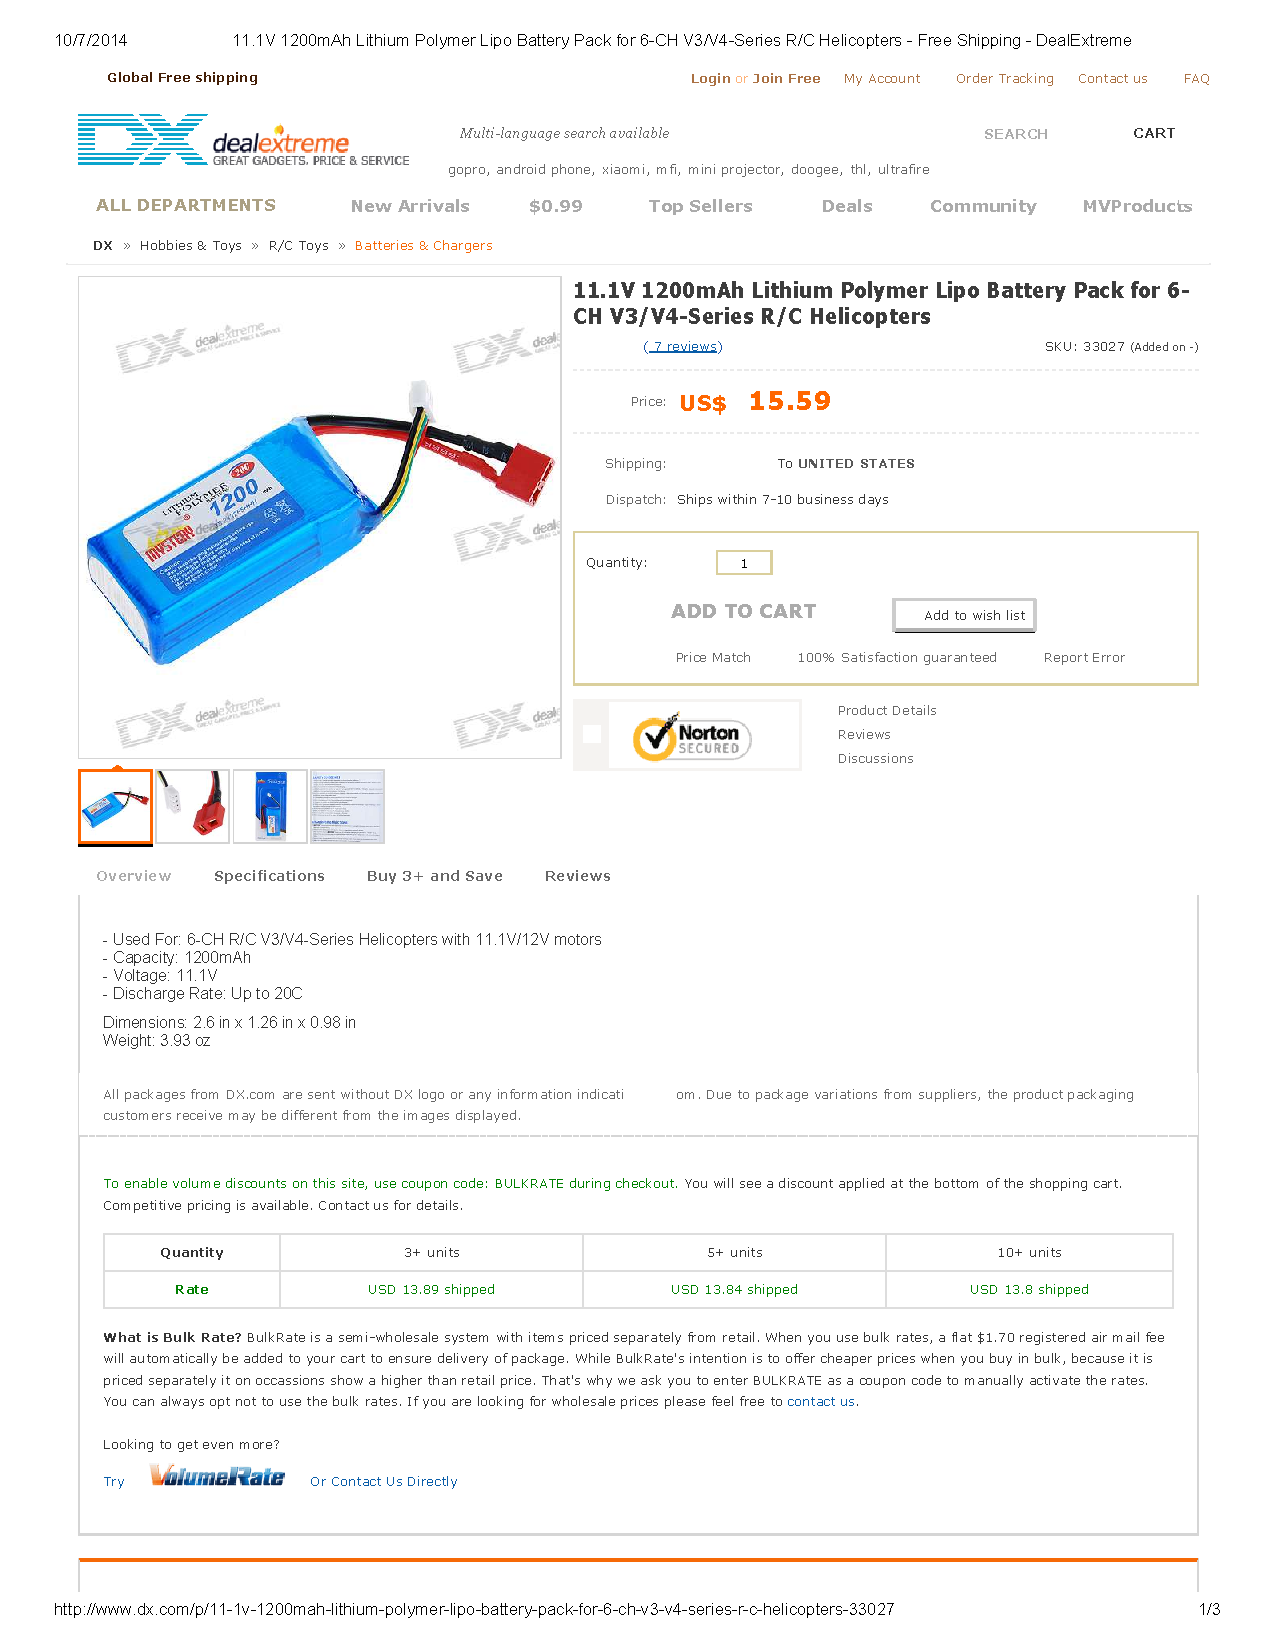
\includepdf[pages = {1}]{Lab6Graphics/Battery.pdf}
	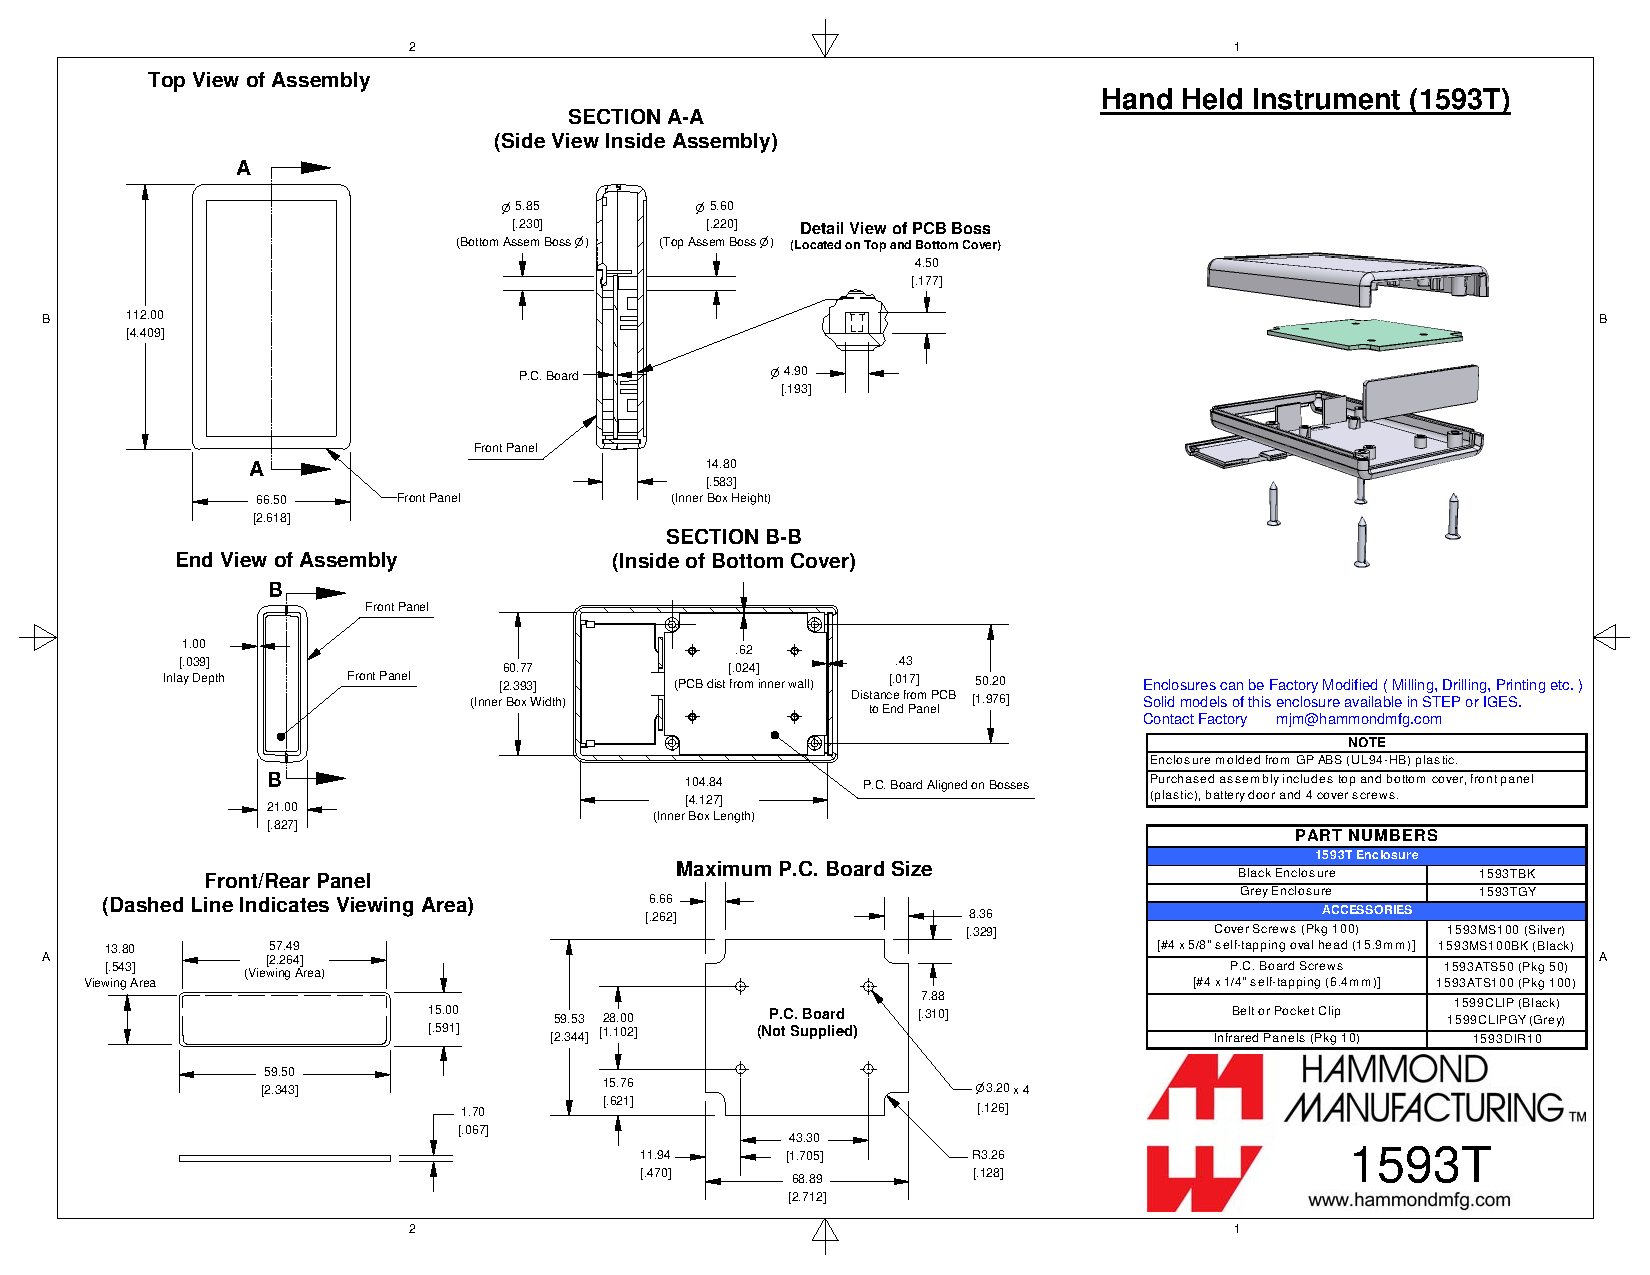
\includepdf[pages = {1}]{Lab6Graphics/BoxDrawings.pdf}
	\begin{figure}[h]
		\includegraphics[keepaspectratio, width = \textwidth]{Lab6Graphics/Lab6SChematic.png}
	\end{figure}
	
%----------------------------------------------------------------------------------------
%	SECTION 3 Software Design
%----------------------------------------------------------------------------------------
%\section{Software Design}

%----------------------------------------------------------------------------------------
%	SECTION 4 Measurement Data
%----------------------------------------------------------------------------------------
\section{Measurement Data}
	The battery was chosen because it provides 11.1V and has a capacity of 1200 mAh meaning it would be able to drive our motor for at least 4 hours of continuous use. The motor current measured during lab 4 was 209 mA at it's highest point. Assuming a worst case of 250 mA draw from the motors, 4 hours of continuous use would require 1000mAh. The motor is also rated to be supplied from 6 to 24 V and the power regulator upper limit is well above the 11.1 V level of the battery. The only other effect with this battery versus performance we measured in class is the higher voltage will cause the motor to higher possible RPM than what we saw in class and will likely require re-tuning of our I control.
%----------------------------------------------------------------------------------------
%	SECTION 5 Analysis and Discussion
%----------------------------------------------------------------------------------------
\section{Analysis and Discussion}
	The following tests should be run in order and start with an unpopulated board with components added as each test case requires. The testing procedure we would suggest is as follows:
	\begin{enumerate}
		\item %test case 1
			\textbf{Tachometer Input Circuit:} Populate the components of the Tachometer circuit. These components consist of R2, R3, R7, R8, R9, D2, D3, and the OPA2350N. After verifying components are in the correct locations and orientations, connect a power supply to the \textbf{+3V3} and \textbf{GND} lines and attach a signal generator to the \textbf{TACH} test point. Be sure to limit the current output of the power supply to 500 mA for the safety of the components. Generate a sine wave oscillating between $\pm5V$ and verify that the output from the op-amp at the \textbf{INPUT} test point is a square wave oscillating between 0 and 3.3 V.
		\item %test case 2
			\textbf{Motor Output Circuit:} Populate the components of the Motor circuit. These components consist of R1, D1, the TIP120 transistor, the headers for attaching the motor, and a test motor. After verifying components are in the correct location and orientations, connect a power supply to the \textbf{+11V1} and \textbf{GND} lines and attach a signal generator to the \textbf{PWM} test point. Be sure to limit the current output of the power supply to 1 A for the safety of the components being tested. Generate a square wave oscillating between 0 and 5 V and varying the duty cycle of the signal. Verify that the output angular velocity of the motor is changing correctly to the changing duty cycle.
		\item %test case 3
			\textbf{Power Regulation Circuit:} Populate the components of the Power Regulation circuit. These components consist of C1, C2, and the LM2937-3.3. After verifying components are in the correct locations and orientations, connect a power supply to the \textbf{+11V1} and \textbf{GND} lines. Be sure to limit the current output of the power supply to 0.5 A for the safety of the components being tested. Turn on the power supply and verify that the \textbf{+3V3} line is at +3.3 V.
	\end{enumerate}


\end{document}